\documentclass[11pt]{scrartcl}
\usepackage[sexy]{evan}
\usepackage{graphicx}
\usepackage[spanish]{babel}
\graphicspath{ {./images/} }

\usepackage{answers}
\Newassociation{hint}{hintitem}{all-hints}
\renewcommand{\solutionextension}{out}
\renewenvironment{hintitem}[1]{\item[\bfseries #1.]}{}

\usepackage{venndiagram,multicol,hyperref,graphicx,array,xskak}

\begin{document}
\title{Principio Extremo}
\author{Ricardo Largaespada}
\date{03 Agosto 2024}

\maketitle
\section{Introducción}

El principio extremo en combinatoria es una herramienta poderosa utilizada para resolver problemas en diversas áreas de la matemática, especialmente en combinatoria y teoría de grafos. Este principio se basa en la idea de analizar elementos extremos de un conjunto, como los elementos máximos o mínimos, y utilizar sus propiedades para derivar conclusiones generales sobre el conjunto completo.

\subsection*{Definición}

En términos generales, el principio extremo establece que en cualquier conjunto finito de elementos, siempre existen elementos extremos, es decir, elementos que son mínimos o máximos en algún sentido. Al enfocarse en estos elementos extremos, a menudo es posible simplificar y resolver problemas complejos.

\subsection*{Aplicaciones Comunes}

El principio extremo se utiliza en una variedad de contextos combinatorios, tales como:

\begin{itemize}
    \item \textbf{Grafos}: Determinar propiedades de grafos, como caminos, ciclos.
    \item \textbf{Geometría Discreta}: Analizar configuraciones de puntos y rectas en el plano.
    \item \textbf{Teoría de Números}: Resolver problemas relacionados con conjuntos de números y sus propiedades.
    \item \textbf{Teoría de Conjuntos}: Probar la existencia de subconjuntos con propiedades específicas.
\end{itemize}

\subsection*{Ejemplos Clásicos}

\begin{itemize}
    \item \textbf{Teorema de Erdős–Szekeres}: En cualquier secuencia de \(n^2 + 1\) números distintos, siempre existe una subsecuencia creciente de longitud \(n+1\) o una subsecuencia decreciente de longitud \(n+1\).
    \item \textbf{Principio de Casillas }: Si se distribuyen más de \(n\) elementos en \(n\) compartimentos, al menos un compartimento contendrá más de un elemento.
\end{itemize}

\subsection*{Método de Prueba}

El uso del principio extremo generalmente sigue estos pasos:

\begin{enumerate}
    \item Identificar el conjunto de elementos que se está considerando.
    \item Determinar una propiedad extrema relevante (mínimo, máximo, etc.).
    \item Analizar las consecuencias de la existencia de este elemento extremo.
    \item Utilizar estas consecuencias para resolver el problema original.
\end{enumerate}

El principio extremo es una herramienta fundamental en la resolución de problemas combinatorios. Al centrarse en elementos extremos de un conjunto, es posible simplificar y abordar problemas que de otro modo serían complejos. La habilidad de identificar y utilizar estos elementos extremos es una parte esencial del arsenal de cualquier matemático.\\

Ahora algunos ejemplos:

\begin{example}[Leningrado 1988]
    Algunas fichas están en un tablero de ajedrez. A cada segundo, cada una de las fichas se mueve a una casilla vecina (lado en común). Después de mucho tiempo, se verificó que cada ficha había pasado por todas las casillas del tablero exactamente una vez y había vuelto a su casilla inicial. Pruebe que existió un momento en que todas las fichas estaban fuera de su casilla inicial.
\end{example}
Solución. Sea \(P\) la primera ficha que volvió a su posición inicial. Un movimiento antes de que vuelva a su casilla, cada uno de las otras fichas debe haber hecho un movimiento. De hecho, si esto no fuera verdad, \(P\) no podría haber pasado por todas las casillas del tablero. De este modo, este será el momento en que todas las fichas estarán en casillas diferentes de las iniciales.

\begin{example}[Teorema de Sylvester]
    Un conjunto finito \(S\) de puntos en el plano posee la propiedad de que cualquier línea que pasa por dos de estos puntos también pasa por un tercero. Pruebe que todos los puntos están sobre una línea.
\end{example}

\begin{center}
    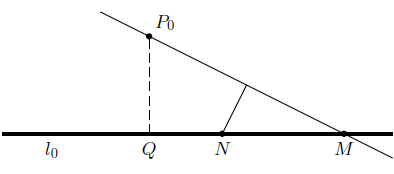
\includegraphics[scale=1]{images/clase_13_silvestre.png}
\end{center}

Solución. Sea \(L\) el conjunto de todas las líneas que pasan por al menos dos puntos de \(S\). Ahora sean \(P_0 \in S\) y \(l_0 \in L\) tales que la distancia entre \(P_0\) y \(l_0\) es la menor posible, pero diferente de cero. Sea \(Q\) la proyección de \(P_0\) sobre \(l_0\). Como la línea \(l_0\) pasa por tres de ellos, al menos dos de ellos \(N\) y \(M\) están en la misma semi-línea (en relación a \(Q\)). Suponga que \(N\) es el más próximo de \(Q\); de este modo, la distancia entre \(N\) y la línea \(P_0M\) es menor que la mínima. Contradicción.\\

\begin{example}[Leningrado 1989]
    Dado un número natural \(k\) mayor que 1, pruebe que es imposible colocar los números \(1, 2, \ldots, k^2\) en un tablero \(k \times k\) de forma que todas las sumas de los números escritos en cada fila y columna sean potencias de 2.
\end{example}
Solución. Suponga que es posible hacer tal distribución para algún entero positivo \(k\). Además, sea \(2^n\) la menor de las sumas. Debemos tener:
\[
2^n \leq 1 + 2 + \cdots + k = \frac{k(k+1)}{2}.
\]
Como \(2^n\) es la menor potencia, \(2^n\) divide la suma de los elementos en cualquier fila, por lo tanto, divide la suma de todos los elementos del tablero. Así:
\[
2^n \mid \frac{k^2(k^2 + 1)}{2}.
\]
Como \(k^2\) y \(k^2 + 1\) tienen paridades opuestas, \(2^{n+1}\) debe dividir solo uno de ellos. En cualquier caso, tenemos \(2^{n+1} \leq k^2 + 1\). Esto contradice la primera desigualdad encontrada.

\begin{example}[San Petersburgo 1998]
    En cada una de diez hojas de papel están escritas diversas potencias de 2. La suma de los números en cada una de las hojas es la misma. Muestre que algún número aparece al menos 6 veces.
\end{example}
Solución. Sea \(N\) la suma común, y \(n\) el mayor entero tal que \(2^n \leq N\). Suponga que cada potencia solo ocurre como máximo 5 veces. De ahí,
\[
5(1 + 2 + \cdots + 2^n) = 5(2^{n+1} - 1) < 10N.
\]
Y esto genera una contradicción.

\Opensolutionfile{all-hints}

\section{Problemas Propuestos}

\begin{problem}
    Dado un conjunto de \(n\) puntos en el plano, no todos en una misma recta, existe una recta que pasa por exactamente dos de esos puntos.
    \begin{hint}
    Si dibujas todas las rectas posibles a través de pares de puntos, considera cuántos puntos pueden estar en la misma recta.
    \end{hint}
\end{problem}
    
\begin{problem}
Ocho equipos de fútbol participan en un torneo de una vuelta (cada equipo juega una vez contra cada uno de los demás).  No hay empates.  Demostrar que es posible que al final del torneo haya 4 equipos, digamos $A$, $B$, $C$ y $D$, de modo que $A$ haya derrotado a $B$, $C$ y $D$, $B$ haya derrotado a $C$ y $D$, y $C$ haya derrotado a $D$.
    \begin{hint}
    ¿Cuántos enfrentamientos hay en el torneo?
    \end{hint}
\end{problem}
    
\begin{problem}
    Hay 20 países en un planeta. Se sabe que entre cualquier tres de estos países, siempre hay dos sin relaciones diplomáticas. Pruebe que existen, como máximo, 200 embajadas en este planeta.
    \begin{hint}
    Considera cómo se pueden maximizar las relaciones diplomáticas.
    \end{hint}
\end{problem}

\begin{problem}
    Todo participante de un torneo juega con cada uno de los otros participantes exactamente una vez. Después del torneo, cada jugador hace una lista con los nombres de todos los jugadores vencidos por él y de todos los que fueron vencidos por los jugadores que él venció. Sabiendo que en este torneo no hay empates, pruebe que existe un jugador cuya lista contiene el nombre de todos los otros jugadores.
    \begin{hint}
    Piensa en el concepto de grafo dirigidos.
    \end{hint}
\end{problem}

\begin{problem}
    Considere tres escuelas, cada una con \(n\) alumnos. Cada estudiante tiene en total \(n + 1\) amigos en las otras dos escuelas donde él no estudia. Pruebe que es posible seleccionar un estudiante de cada escuela de tal forma que los tres se conozcan mutuamente.
    \begin{hint}
    Usa el teorema de la amistad.
    \end{hint}
\end{problem}

\begin{problem}
    En cada punto de la cuadrícula del plano se coloca un entero positivo. Cada uno de esos números es el promedio aritmético de sus cuatro vecinos. Muestre que todos los números son iguales.
    \begin{hint}
    El mayor de los números es mayor o igual que el promedio.
    \end{hint}
\end{problem}

\Closesolutionfile{all-hints}

\section{Sugerencias y Soluciones}
\begin{enumerate}
\input{all-hints.out}
\end{enumerate}

\section*{Teorema de Erdős–Szekeres}

\begin{theorem}
En cualquier secuencia de \(n^2 + 1\) números distintos, siempre existe una subsecuencia creciente de longitud \(n + 1\) o una subsecuencia decreciente de longitud \(n + 1\).
\end{theorem}

Este teorema es una declaración poderosa sobre la estructura interna de cualquier secuencia suficientemente larga de números distintos. Es una aplicación del principio de casillas.

\begin{proof}
    Considere una secuencia de \(n^2 + 1\) números distintos \(a_1, a_2, \ldots, a_{n^2+1}\).
    
    Definimos dos funciones \(L(i)\) y \(M(i)\) para cada \(1 \leq i \leq n^2 + 1\):
    \begin{itemize}
        \item \(L(i)\) es la longitud de la subsecuencia creciente más larga que termina en \(a_i\).
        \item \(M(i)\) es la longitud de la subsecuencia decreciente más larga que termina en \(a_i\).
    \end{itemize}
    
    Observamos que \(1 \leq L(i), M(i) \leq n + 1\) porque si alguna de estas longitudes fuera mayor que \(n + 1\), tendríamos una subsecuencia creciente o decreciente de longitud mayor a \(n + 1\).
    
    Ahora, consideramos el par \((L(i), M(i))\) para cada \(1 \leq i \leq n^2 + 1\). Cada par \((L(i), M(i))\) puede tener \(n + 1\) valores posibles para cada componente, lo que nos da un total de \((n + 1) \times (n + 1) = n^2 + 2n + 1\) posibles pares diferentes.
    
    Sin embargo, tenemos \(n^2 + 1\) elementos en nuestra secuencia, lo que significa que necesariamente alguno de los valores \((L(i), M(i))\) se repetirá más de una vez por el principio de Dirichlet.
    
    Supongamos que no existe una subsecuencia creciente de longitud \(n + 1\) ni una subsecuencia decreciente de longitud \(n + 1\). Entonces, \(1 \leq L(i), M(i) \leq n\) para todos los \(i\), lo que da un total de \(n \times n = n^2\) posibles pares diferentes.
    
    Pero, como tenemos \(n^2 + 1\) elementos, debe existir al menos un par repetido, lo cual contradice nuestra suposición de que no existen subsecuencias crecientes o decrecientes de longitud \(n + 1\).
    
    Por lo tanto, siempre debe existir una subsecuencia creciente de longitud \(n + 1\) o una subsecuencia decreciente de longitud \(n + 1\).
\end{proof}

\subsection*{Ejemplo}

Consideremos \(n = 3\). Según el teorema, en cualquier secuencia de \(3^2 + 1 = 10\) números distintos, siempre existe una subsecuencia creciente de longitud \(3 + 1 = 4\) o una subsecuencia decreciente de longitud \(3 + 1 = 4\).

Por ejemplo, para la secuencia \(1, 9, 3, 8, 2, 7, 4, 6, 5, 10\):
\begin{itemize}
    \item La subsecuencia creciente \(1, 3, 4, 5, 10\) tiene longitud 5.
    \item La subsecuencia decreciente \(9, 8, 7, 6\) tiene longitud 4.
\end{itemize}

En este caso, ambos tipos de subsecuencia existen y cumplen con el teorema.

\end{document}